\documentclass[11pt]{article}
\usepackage {tikz}
\usetikzlibrary{automata, positioning}

\usepackage{mdframed}
\usepackage{amsmath,amsthm,amssymb}
\newmdtheoremenv{theo}{Theorem}

\usepackage{enumerate}
\usepackage{fullpage,amsmath,amssymb}
\usepackage[colorlinks=true,citecolor=blue,linkcolor=blue]{hyperref} % for href links, and also makes \ref and \eqref clickable in the PDF

\newcommand{\QuasiP}{\mathsf{QuasiP}}

\newcommand{\TIME}{\mathsf{TIME}}
\newcommand{\N}{\mathbb{N}}
\renewcommand{\P}{\mathsf{P}}
\newcommand{\NP}{\mathsf{NP}}
\newcommand{\poly}{\mathrm{poly}}
\newcommand{\SAT}{\textsc{Sat}}
\newcommand{\sat}{\SAT}
\newcommand{\tsat}{3\sat}
\newcommand{\dnfsat}{\textsc{DNF-\sat}}
\newcommand{\cnfsat}{\textsc{CNF-\sat}}
\newcommand{\pmat}{\textsc{Perfect-Matching}}
\newcommand{\iset}{\textsc{Independent-Set}}
\newcommand{\cpc}{\textsc{Cellphone-Capacity}}

\usepackage{fancyhdr}
\fancypagestyle{firststyle}
{
   \fancyhf{}
   \fancyhead[C]{Copyright \copyright\ \today, David Doty}
}



\title{Homework 2 -- ECS 220, Spring 2020}
\date{}

\begin{document}
\maketitle
\thispagestyle{firststyle}
\vspace{-2.0cm}




%\documentclass[11pt]{article}
\usepackage{listings}
\usepackage{xcolor}
\definecolor{codegreen}{rgb}{0,0.6,0}
\definecolor{codegray}{rgb}{0.5,0.5,0.5}
\definecolor{codepurple}{rgb}{0.58,0,0.82}
\definecolor{backcolour}{rgb}{0.95,0.95,0.92}
\lstset{
    language=Python,
    keepspaces=true,
    numbers=left,
    backgroundcolor=\color{backcolour},
    commentstyle=\color{codegreen},
    basicstyle=\ttfamily,
    otherkeywords={self,True,False,yield},
    keywordstyle=\ttfamily\color{blue!90!black},
    %basicstyle=\footnotesize,
    keywords=[3]{ttk},
    keywordstyle={[2]\ttfamily\color{orange!80!orange}},
    keywordstyle={[3]\ttfamily\color{red!80!orange}},
    emph={MyClass,__init__},
    emphstyle=\ttfamily\color{red!80!black},
    stringstyle=\color{green!80!black},
    showstringspaces=false
}
\usepackage{enumerate}
\usepackage{fullpage,amsmath,amssymb,graphicx}
\usepackage[colorlinks=true,citecolor=blue,linkcolor=blue]{hyperref} % for href links, and also makes \ref and \eqref clickable in the PDF
\newcommand{\QuasiP}{\mathsf{QuasiP}}
\newcommand{\TIME}{\mathsf{TIME}}
\newcommand{\N}{\mathbb{N}}
\newcommand{\Z}{\mathbb{Z}}
\renewcommand{\P}{\mathsf{P}}
\newcommand{\NP}{\mathsf{NP}}
\newcommand{\poly}{\mathrm{poly}}
\newcommand{\SAT}{\textsc{Sat}}
\newcommand{\sat}{\SAT}
\newcommand{\dnfsat}{\textsc{DNF-\sat}}
\newcommand{\cnfsat}{\textsc{CNF-\sat}}
\newcommand{\pmat}{\textsc{Perfect-Matching}}
\newcommand{\iset}{\textsc{Independent-Set}}
\newcommand{\cpc}{\textsc{Cellphone-Capacity}}
\usepackage{fancyhdr}
\fancypagestyle{firststyle}
{
   \fancyhf{}
   \fancyhead[C]{Copyright \copyright\ \today, David Doty}
}
\title{Homework 3 -- ECS 220, Winter 2020}
\date{}
\begin{document}
\maketitle
\thispagestyle{firststyle}
\vspace{-2.0cm}

\section*{Really independent sets}
    \begin{quote}
    Given a graph $G = (V,E)$, say that a subset $S \subseteq V$ is \emph{really independent} if there are no $u,v \in S$ that are two or fewer steps apart in the graph---that is, if for all $u,v \in S$, the length of the shortest path
    between $u$ and $v$ is at least 3.
    The problem \textsc{ReallyIndependentSet} takes a graph $G$ and an integer $k$ as input, and asks if $G$ has a really independent set of size $k$ or more.
    Prove that \textsc{ReallyIndependentSet} is $\NP$-complete.
    \end{quote}
\end{document}\newpage
%
\subsection*{How to mail a matrix. (Textbook problem 2.18)}
    \begin{quote}
    Given a graph $G = (V, E)$ with $|V| = n$ vertices and $|E| = m$ edges, how many bits do we need to specify the adjacency matrix, and how many do we need to specify an adjacency list? Keep in mind that it takes $\log n$ bits to specify an integer between $1$ and $n$. When are each of these two formats preferable?

    In particular, compare sparse graphs where $m = O(n)$ with dense graphs where $m = \Theta(n^2)$. How do things change if we consider a multigraph, like the graph of the K\"{o}nigsberg bridges, where there can be more than one edge between a pair of points?
    \end{quote}

    \begin{solution}
        
        First of all, we know that the space complexity of an adjacency matrix is $O(n^2)$, while that of an adjacency list is $O(n+m)$. In an adjacency matrix we only need one bit to specify if there is an edge between node $i$ and node $j$($A_{ij} = 0$ for no edge between node $i$ and node $j$, $A_{ij} = 1$ for an edge between them), so we'll need $n^2$ bits to specify an adjacency matrix. In the adjacency list we need to store the index of the node, so $log(n)$ bits are required for each node. Therefore, we need $(n+m)log(n)$ bits to specify an adjacency list.
        
        When a graph is sparse, for example $m = O(n)$, the adjacency matrix is still going to take $n^2$ while wasting a lot of space to store no connection between nodes. In the mean time, the adjacency list can store connections more efficiently($O(n+n)$ will still be $O(n)$), so when a graph is sparse, a list representation should be preferable. On the other hand, if a graph is dense, both the adjacency matrix and the adjacency list need $O(n^2)$. But we can check the connection between two points in constant time in adjacency matrix, so the adjacency matrix is preferable when the graph is dense.
        
        If a multigraph is considered, a single bit is not enough to store the connection between nodes in a adjacency matrix. If there are two edges between node $i$ and node $j$, $A_{ij}$ should be 2. So each element in the matrix takes more bits. Assume there are at most $k$ edges between any two nodes in the graph, it should take $n^2log(k)$ bits to specify the matrix, and the adjacency matrix is going to look like a weighted adjacency matrix. There will be duplicated nodes in the adjacency list for those edges connecting the same nodes. But it still takes $(n+m)log(n)$ to specify the adjacency list.
        
    \end{solution}\newpage
\documentclass[11pt]{article}

%\usepackage[nosol]{optional}
\usepackage[sol]{optional}
\usepackage{listings, ../listings-rust/listings-rust}

\newcommand{\N}{\mathbb{N}}
\newcommand{\Z}{\mathbb{Z}}
\renewcommand{\P}{\mathsf{P}}
\newcommand{\NP}{\mathsf{NP}}
\newcommand{\SAT}{\textsc{Sat}}

\usepackage{enumerate,color,comment}
\usepackage{graphicx}

% For proof.
\usepackage{amsmath,amsthm,amssymb}

\usepackage{fullpage,amsmath,amssymb}
\usepackage[colorlinks=true,citecolor=blue,linkcolor=blue]{hyperref} % for href links, and also makes \ref and \eqref clickable in the PDF


\usepackage{fancyhdr}
\fancypagestyle{firststyle}
{
   \fancyhf{}
   \fancyhead[C]{Copyright \copyright\ \today, David Doty}
}


\title{Homework 4 \opt{sol}{Solutions} -- ECS 220, Winter 2020}
\date{}
\newtheorem{theorem}{Theorem}
\begin{document}
\maketitle
\thispagestyle{firststyle}
\vspace{-2.0cm}

\newcommand{\II}{\#2}
\newcommand{\III}{\#3}
\newcommand{\V}{\#5}
\newcommand{\VII}{\#7}
\newcommand{\XI}{\#11}
\newcommand{\XIII}{\#13}
\newcommand{\XVII}{\#17}

\section{Programming with Fractions}
    The late John Conway invented the following programming language that is defined by a finite sequence of fractions.
    
    Consider the following example:
    
    \[
    \frac{33}{14} \quad
    \frac{21}{22} \quad
    \frac{13}{7} \quad
    \frac{13}{11} \quad
    \frac{26}{85} \quad
    \frac{34}{65} \quad
    \frac{1}{13} \quad
    \frac{1}{17} \quad
    \frac{10}{3} \quad
    \frac{7}{1}
    \]
    
    We start from the value $n=6=2^1 3^1$. At each step, we find the first fraction $f=\frac{p}{q}$ such that $q$ divides $n$ (i.e., such that $n \cdot f$ is an integer), and then replace $n$ by $n \cdot f$. If there is no such $f$, the program halts.
    
    For this example, the sequence of values produced will include the infinite subsequence $2^1 3^1$, $2^1 3^2$, $2^2 3^3$, $2^3 3^5$, $2^5 3^8$, $2^8 3^{13}$, $\ldots$.
    Whenever $n$ is only divisible by $2$ and $3$, the exponents will be adjacent Fibonacci numbers.
    
    Prove why this program outputs the Fibonacci numbers in this way, or instead find your own program that outputs Fibonacci numbers and prove it works.
    
    \textbf{Hint:} you can view this computation as a special type of counter machine.
    See section 7.6.2 in the text for more examples.

\section*{Solution}

We shall setch this model to a counter machine. 
In this machine we use 7 counter to represent the number of each primes(i.e. $2, 3, 5, 7, 11, 13, 17$) that can be decomposed from each step.
In the following proof, we would use notation $\#x$ to refer to the counter that is counting the number of $x$.
Then the step of switching from $n$ to $n\cdot f$ would become increase counters that are in $p$ and decrease the counters that are in $q$.

In this machine, we add the conditions and assertions to each edge.
In this way, we showed that given input of the form $2^s3^t$, the output put has to be in the same form.
Notice the asserts and branches in the graph that guarantees that at accepting state $\V = \VII = \XI = \XII = \XVII = 0$.

Not let's proof that this machine actually generates a Fib sequence.
Since we already known that the initial case is $s = 1, t = 1$, all we need to proof is that, given input $2^s3^t$, the output would be $2^t3^{s+t}$

\begin{theorem}
    Given input $2^s3^t$, $s < t$, the output would be $2^t3^{s+t}$
\end{theorem}

\begin{proof}

    We shall walk through the machine to proof that.
    \begin{enumerate}
        \item Initial input has counter value $\II = s, \III = t$, all other counters are zero.
        \item We would be looping at state $\frac{10}{3}$ until we have $\V = t, \II = s + t, \III = 0$, i.e. there is no $3$ left. 
        \item At state $\frac{7}{1}$, since $q = 1$, it is always executed once and leave us $\VII = 1$, everything else unchanged.
        \item Then we would be looping between state $\frac{33}{14}$ and state $\frac{21}{22}$. These two states aim to wipe out all the $2$. If $\II$ becomes zero at state $\frac{33}{14}$, then it comes to state $\frac{13}{11}$ with $\XI = 1, \III = s + t$; If $\II$ becomes zero at state $\frac{21}{22}$, then it comes to state $\frac{13}{7}$ with $\VII = 1, \III = s + t$.
        \item Either state $\frac{13}{11}$ or state $\frac{13}{7}$ will only executed once and leave us $\XIII = 1, \III = s + t$. 
        \item Then we would be looping between state $\frac{34}{65}$ and state $\frac{26}{85}$. These two states aim to wipe out all the $5$. If $\V$ becomes zero at state $\frac{34}{65}$, then it comes to state $\frac{1}{17}$ with $\XVII = 1, \II = t, \III = s + t$; If $\V$ becomes zero at state $\frac{26}{85}$, then it comes to state $\frac{1}{13}$ with $\XIII = 1, \II = t, \III = s + t$;
        \item Either state $\frac{1}{17}$ or state $\frac{1}{13}$ will only executed once and leave us $\II = t, \III = s + t$. 
        \item Finally it returns to the accepting state $2^t3^{s+t}$ with $\II = t, \III = s + t$. 
    \end{enumerate}
\end{proof}
 \begin{figure}[h]
        \centering
        \begin{tikzpicture}[shorten >=1pt,node distance=2cm,on grid,auto, semithick,
        el/.style = {inner sep=7pt, align=left, sloped}] 
        %\tikzstyle{every node} = [circle, draw]
        \node [state, scale=2,el,label={[blue,align=left]above:$\#2++$\\$\#3--$}] (2) {$\frac{10}{3}$};
        \node [state, initial above,accepting, scale=2,position=40:1 cm from 2,] (1) {$2^s 3^t$};
        \node [state, scale=2, position=200: 2cm from 2,el,label={[blue,align=left]above:$\#7++$}] (3) {$\frac{7}{1}$};
        \node [state, scale=2, position=-20: 2cm from 2,el,label={[blue,align=left]right:$\#13--$}] (4) {$\frac{1}{13}$};
        \node [state, scale=2, below of=3,el,label={[blue,align=left]left:$\#3++$\\$\#11++$\\ $\#2--$\\$\#7--$}] (5) {$\frac{33}{14}$};
        \node [state, scale=2, position=0:0.9cm from 5,el,label={[blue,align=left]above:$\#3++$\\$\#7++$\\ $\#2--$\\$\#11--$}] (6) {$\frac{21}{22}$};
        \node [state, scale=2, right of=6,el,label={[blue,align=left]right:$\#17--$}] (7) {$\frac{1}{17}$};
        \node [state, scale=2, below of=5,el,label={[blue,align=left]left:$\#13++$\\$\#11--$}] (8) {$\frac{13}{11}$};
        \node [state, scale=2, position=0:0.9cm from 8,el,label={[blue,align=left]left:$\#13++$\\$\#7--$}] (9) {$\frac{13}{7}$};
        \node [state, scale=2, below right of=9,el,label={[blue,align=left]below:$\#2++$\\$\#17++$\\ $\#5--$\\$\#13--$}] (11) {$\frac{34}{65}$};
        \node [state, scale=2, position=0: 2.6cm from 9,el,label={[blue,align=left]right:$\#2++$\\$\#13++$\\ $\#5--$\\$\#17--$}] (10) {$\frac{26}{85}$};
        
       
    \path[->]
        (1)  edge[cfgedge, bend right=10] (2)
        (2)  edge[cfgedge, bend right=10] node[el,above] {$\#3=0$} (3)
        (2)  edge[in=240, out=-60,loop] node[el,above] {$\#3\ne0$} (2)
        (3)  edge[cfgedge] node [el,below] {$\#7=1$} (5)
        (5)  edge[cfgedge,bend left=20] node [el,above] {$\#2\ne0$} (6) 
        (6)  edge[cfgedge,bend left=20] node [el,below] {$\#2\ne0$} (5)
    %    (5)  edge[in=150, out=210,loop] node[el,above] {$\#2\ne0$ \\ $\#7\ne0$} (5)
        (5)  edge[cfgedge] node [el,below] {$\#2=0$ } (8)
        (6)  edge[cfgedge] node [el,above] {$\#2=0$ } (9)
        (8)  edge[cfgedge,bend right=30] node [el,above] {$\#13=1$} (11)
        (9)  edge[cfgedge,bend right=10] node [el,above] {$\#13=1$} (11)
        (11)  edge[cfgedge,bend right=20] node [el,below] {$\#5\ne0$} (10)
        (10)  edge[cfgedge,bend right=20] node [el,below] {$\#5\ne0$} (11)
        (11)  edge[cfgedge] node [el,below] {$\#5=0$} (7)
        (10)  edge[cfgedge] node [el,below] {$\#5=0$} (4)
        (7)  edge[cfgedge]  (1)
        (4)  edge[cfgedge]  (1);
        \end{tikzpicture}
        \caption{Directed graph $G$}
        \label{fig:graph1}
      \end{figure}


\end{document}\newpage
\section*{Crossover logic}
    \begin{quote}
    Complete the crossover gadget of Figure 5.11, and hence the reduction from
    $\textsc{Circuit-Sat}$ to $\textsc{Planar-Circuit-Sat}$,
    by designing a \emph{planar} circuit of AND, OR, and NOT gates that implements an XOR gate, 
    where
    the input and output gates should be \emph{accessible to the outer region} so that they can actually be wired up to other subcircuits in the large circuit without a wire crossing.
    \end{quote}

    To implement an \texttt{xor} gate, the general idea is that $a \texttt{ xor } b = !((!a \wedge !b) \vee (a \wedge b))$.
    
    The circuit for $a \texttt{ xor } b$ is shown in the next figure. 

    Since there are only 4 possible combinations of $a$ and $b$, without loss of generality, we assumed input $a = 1100$ and $b = 1010$ to list all 4 combinations. 
    The corresponding output for each combination are listed above edges.

    Notice how the upper part is doing $a \wedge b$, left part doing $!a \wedge !b$ and lower left exchanging $!a \wedge !b$ and $b$.
    The right is combining $!a \wedge !b$ and $a \wedge b$ and negating the result to output.

    Now that \texttt{xor} gate is complete, we can copy and paste this circuit to Firgure 5.11, and hence finish the reduction from
    $\textsc{Circuit-Sat}$ to $\textsc{Planar-Circuit-Sat}$.
    However, then the circuit would be large and ugly, so we don't put it up here.

	\begin{center}
	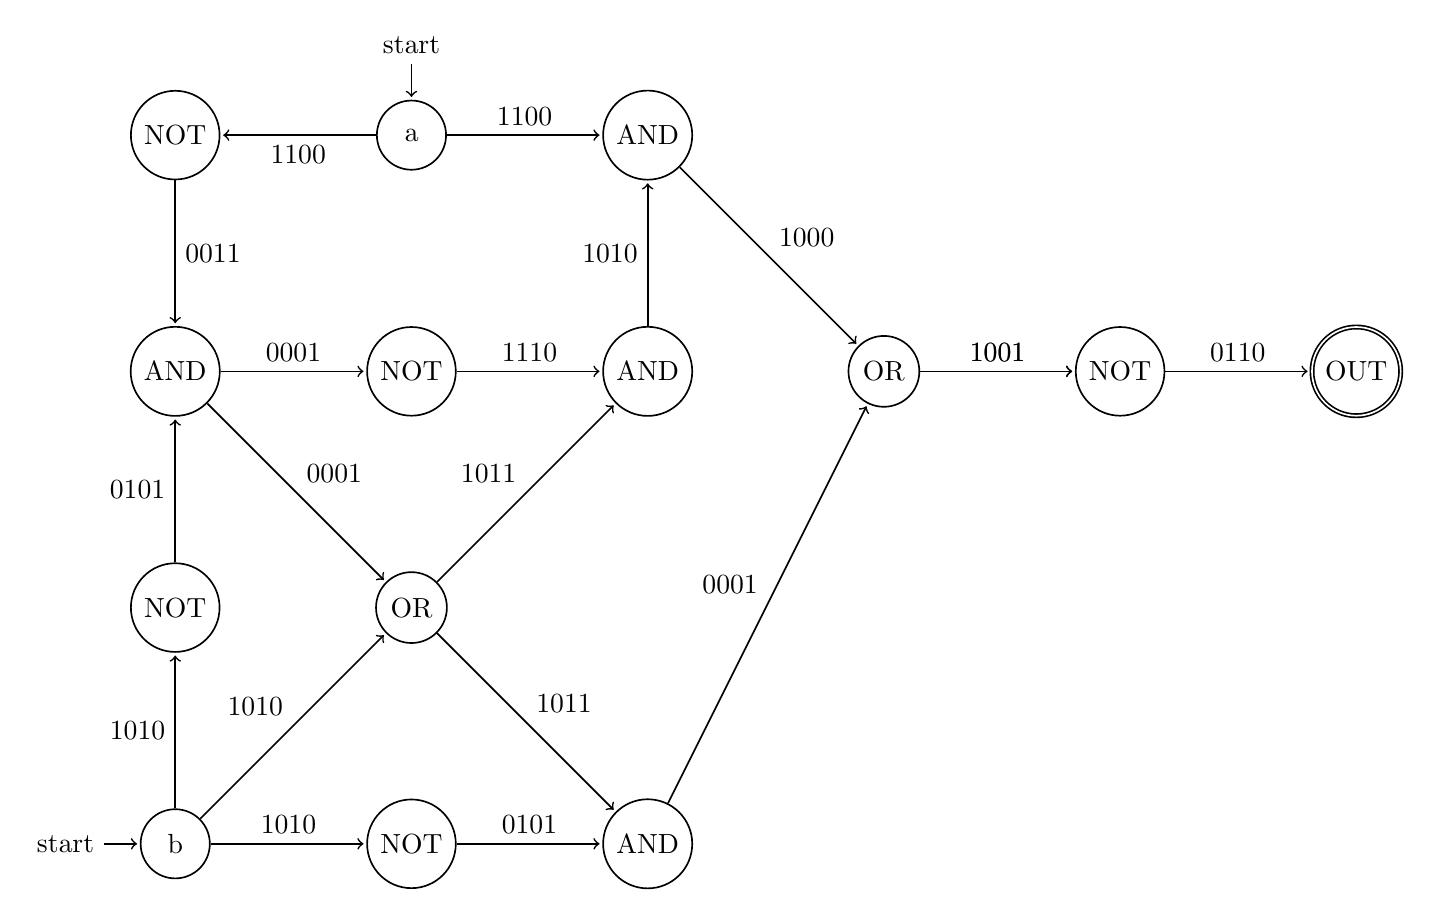
\begin{tikzpicture}[shorten >=1pt,node distance=3cm,on grid,auto, semithick]
		\node[state] 			(nannb) 							{AND};
		\node[state] 			(na) 		[above =of nannb]		{NOT};
		\node[state] 			(nb) 		[below =of nannb]		{NOT};
		\node[state, initial above] (a) 	[right=of na]			{a};
		\node[state, initial] 	(b) 		[below=of nb]	 		{b};
		\node[state] 			(nannbxb) 	[right =of nb]			{OR};
		\node[state]		 	(nnannb) 	[right=of nannb] 		{NOT};
		\node[state]		 	(xb) 		[right=of nnannb] 		{AND};
		\node[state]		 	(xnb) 		[right=of b] 			{NOT};
		\node[state]		 	(xnannb)	[right=of xnb] 			{AND};
		\node[state]			(anb)		[above=of xb]			{AND};
		\node[state]		 	(naxorb) 	[right=of xb] 			{OR};
		\node[state]		 	(axorb) 	[right=of naxorb] 		{NOT};
		\node[state, accepting]	(acc) 		[right=of axorb] 		{OUT};

		\path[->]
			(a) 	edge 		node	{1100} 	(na)
			(b) 	edge 		node	{1010} 	(nb)
			(na) 	edge		node	{0011}	(nannb)
			(nb) 	edge		node	{0101}	(nannb)
			(naxorb)edge		node	{1001}  (axorb)
			(axorb) edge		node	{0110}  (acc)
			(nannb)	edge		node	{0001}  (nnannb)
			(nnannb)edge		node	{1110}	(xb)
			(b)		edge		node	{1010}	(xnb)
			(xnb)	edge		node	{0101}	(xnannb)
			(b) 	edge		node	{1010}	(nannbxb)
			(nannb)	edge		node	{0001}	(nannbxb)
			(nannbxb)	edge	node	{1011}	(xb)
			(nannbxb)	edge	node	{1011}	(xnannb)
			(a)			edge	node	{1100}	(anb)
			(xb)		edge	node	{1010} 	(anb)
			(xnannb)	edge	node	{0001}	(naxorb)
			(anb)		edge	node	{1000}	(naxorb)
			(naxorb)	edge	node	{1001}	(axorb)
			;
	\end{tikzpicture}
	\end{center}
\newpage

\end{document}